\chapter{Available Modules and How to Use Them}
\label{ch:modules}
% ##################################################################################################################

\hfill \textbf{Author:} Andreas Horni, Kai Nagel

\begin{center} 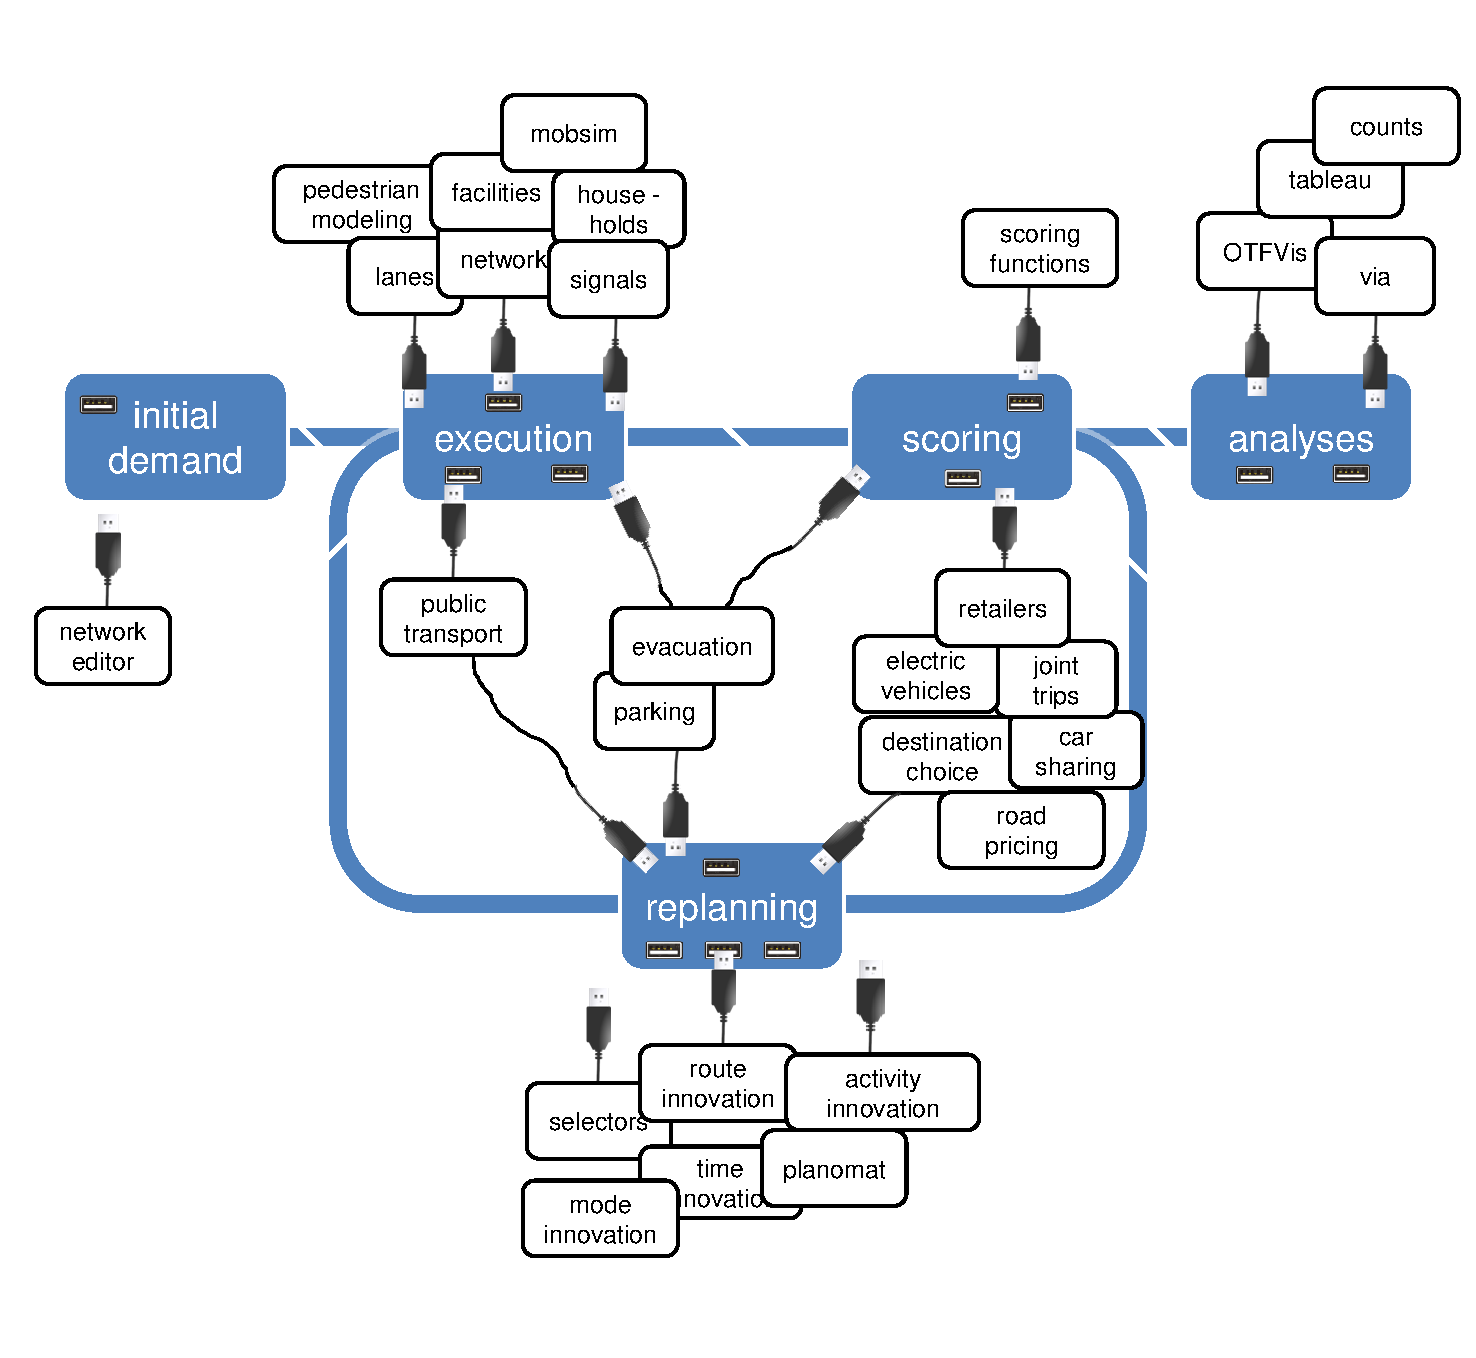
\includegraphics[width=0.5\textwidth, angle=0]{extending/figures/modules.pdf} \end{center}

% ##################################################################################################################
In this chapter you will learn about the possibilities to configure, extend, and customize \gls{matsim} by available functionality. In Chapter~\ref{ch:extensionpoints} you will see how you can hook in your own extensions.

%%\kai{Frage mich im Moment, ob wir diejenigen ``Module'', die man per config aufrufen kann, nicht doch lieber bereits unter ``using'' beschreiben sollten.  Aber vielleicht ist das inzwischen fast egal, und wir sollten lieber Standard-MATSim komplett separat von jeder Art Variation halten.  ???}

% ##################################################################################################################
\section{MATSim Modularity}
\label{sec:matsim-modularity}
\kai{Andreas, haben wir noch eine Chance, diese Ungleichheiten in der Nomenklatur geradezuziehen?  contrib vs extension; PlanStrategy vs StrategyModule; ... }

% ====================================================================================================
\subsection{Levels of Access}
\label{sec:levels-of-access}
\gls{matsim} currently provides four levels of access: using the core only, using core and \glspl{contribution}, writing "scripts in \gls{java}", and finally writing your own \glspl{extension}.

% --------------------------------------------------------------------------------------
\subsubsection{Using the Core Only}
\label{sec:using-core-only}
In order to use the core only, one needs to do the following:
\begin{compactitem}
\item Download a \gls{matsim} release \url{http://sourceforge.net/projects/matsim/files/} or a nightly build \url{http://matsim.org/downloads/nightly} % \kai{url?}.
\item Minimally obtain a network file and an initial plans file.  Small versions can be typed by hand; larger versions should be generated automatically by some computational method.
\item Write or edit a config file.
\item Click on the \gls{matsim} jar file\footnote{This works since winter 2014/15 and should be in the 0.7.0 release.} and follow the instructions. 
\end{compactitem}
We think that the \gls{matsim} core is already quite powerful; for example, the synthetic persons already follow full daily plans with a full daily scoring function and in consequence opening times for activity types, departure time choice, and schedule delay can be investigated.  Also, schedule-based public transit assignment is contained in the core.

% --------------------------------------------------------------------------------------
\subsubsection{Using one or More Contribs}
\label{sec:using-contribs}
\Glspl{contribution} are in a separate part of the repository, separate from the core.  The documentation is not yet fully organized, information about \glspl{contribution} can be found at \url{http://matsim.org/javadoc} or \url{http://www.matsim.org/extensions}.  There are also release versions \kai{check} \ah{gibt es beides am gleichen Ort wie MATSim} and nightly builds \kai{url?}.

In general, \glspl{contribution} should provide main methods with which they can be used.  We might eventually provide clickable jar files here as well, but for the time being the extensions need to be bundled with core \gls{matsim} (and potentially other \glspl{contribution}). As shown at \url{http://www.matsim.org/docs/extensions} the syntax roughly is
\begin{lstlisting}
java -Xmx2000m -cp MATSim.jar:contrib/contrib.jar org.matsim.contrib.run.Main config.xml  
\end{lstlisting}
\kai{Maybe better point to electronic docu?} \ah{siehe url oben}
where
\begin{compactitem}
\item \lstinline$-Xmx2000m$ increases the \gls{java} heap space so that most \gls{matsim} runs fit in
\item \lstinline$MATSim.jar$ needs to be replaced by a relative or absolute path to the \gls{matsim} jar to be used
\item \lstinline$contrib/contrib.jar$ needs to be replaced by a relative or absolute path to the \gls{contribution} jar to be used
\item \lstinline$org.matsim.contrib.run.Main$ needs to be replaced by full \gls{java} class name containing the desired main method (given by the \gls{contribution} documentation)
\item \lstinline$config.xml$ needs to be replaced by a relative or absolute path to a config file, which may contain additional sections specifically for the \gls{contribution}
\end{compactitem}

It is possible to combine several \glspl{contribution} in this way, provided someone has made available a corresponding main method.  This can in principle be done relatively quickly, so persons who want to run studies with combinations of existing \glspl{contribution} but without programming skills can ask someone with those skills and with access to the repository to help.

% --------------------------------------------------------------------------------------
\subsubsection{Writing "Scripts in Java"}
\label{sec:writing-scripts-java}
The \glspl{contribution} are written in a style that they can be plugged into core \gls{matsim} via extension points (see Chapter~\ref{ch:extensionpoints}). If a specific combination or configuration of modules is not (yet) available, one can write it for oneself. The syntax roughly is
\begin{lstlisting}
... main( ... ) {
    // construct the config object:
    Config config = ConfigUtils.xxx(...) ;
    config.xxx().setYyy(...) ;
    ...

    // load and adapt the scenario object:
    Scenario scenario = ScenarioUtils.loadScenario( config ) ;
    scenario.getXxx().doYyy(...) ; // (*)
    ...

    // load and adapt the controler object:
    Controler controler = new Controler( scenario ) ;
    controler.doZzz(...) ; // (**)
    ...

    // run the iterations:
    controler.run() ;
}
\end{lstlisting}
The extension points, especially at \lstinline{(*)} and \lstinline{(**)}, are described in more detail in Chapter~\ref{ch:extensionpoints}.

% --------------------------------------------------------------------------------------
\subsubsection{Writing Your Own Extensions}
\label{sec:writing-your-own-extensions}
If the existing \glspl{contribution} are not sufficient to plug your own study together, the next option is to write your own \gls{extension}.  Again, this should preferably use the extension points described in Chapter~\ref{ch:extensionpoints}, since this is the only way in which an \gls{extension} may later become a \gls{contribution}.  \kai{here is a difference between an extension and a contrib :--)}

%% \paragraph{If none of this is enough}

%% Clearly, it is always possible to download some version of \gls{matsim}, remove all the \lstinline{final} 

% ====================================================================================================
\subsection{The Ideas Behind this Setup}
The setup as described above came out of the observation that an ever growing monolithic \gls{matsim} would eventually overwhelm the core team. Therefore, a set-up was searched where the core team could concentrate on central infrastructure, while specific functionality such as road pricing, multi-modal simulations, signals, additional choice dimensions, or analysis modules could be written and contributed by other people. Clearly, a plug-in architecture had to be the solution, but it took (and still takes) time and effort to make the extension points sufficiently capable and sufficiently robust.  

At the same time, \gls{matsim} is a research platform, and a trait of research is that it investigates innovative questions, which often means that the questions were not foreseen by the designs of the code.  Quite often, scripting languages are the solution to such problems; for example, QGIS or VISUM allows python \cite{...} for plug-ins; EMME allows ???; SUMO allows ??? \kai{traci}.  Scala \cite{...} was discussed for \gls{matsim}, but in the end it was decided to just use Java itself as the scripting language. This has the advantage that persons who are in between core development and \gls{matsim} application do not need to learn two languages, and in addition VSP can continue to teach Java both as an entry point to \gls{matsim} and as a general professional skill.

% ====================================================================================================
\subsection{MATSim Modules}
According to the Merriam-Webster (\url{http://www.merriam-webster.com}), a module is
%
"one of a set of parts that can be connected or combined to build or complete something" 
%
or more specifically
%
"a part of a computer or computer program that does a particular job". 
%
That is, "module" is not a very specific term, and in consequence modules exist in \gls{matsim} at many levels.
%
In the following are some important examples.

%% The basic concept to extend MATSim is the usage of modules. But, please be aware that when it comes to configuring MATSim the term ``module'' is very extensively used such that a clear definition of what is a module and what is not is not available to date. This consequence of organic grows be corrected on the long run, for now, we try to just sort out the different meanings of the word module

%% \kai{Ich bilde mir ein, dass wir das im Kopf schon etwas klarer haben, als es historisch noch aussieht, und würde gerne versuchen, das hier zu kommunizieren.  Ich habe in der Einleitung zu Kap.~\ref{ch:extensionpoints} etwas geschrieben, was man vielleicht inhaltlich auch hier verwenden kann ...}

%% Following different components are called modules.

%% \paragraph{Components in \lstinline|org.matsim|:} % --------------
% ...........................................................................
\paragraph{Config Modules:} % --------------
The config \gls{xml} file uses a syntax of the type
\begin{xml}
<module name="aModule">
    <param name="aParameterForAModule0" value="someValueX" />
    <param name="aParameterForAModule1" value="someValueY" />
</module>
\end{xml}
The config modules loosely correspond to components providing distinct functionality. 

%% residing in the \lstinline|org.matsim| package.  

%% Habe das mal auskommentiert.  Ist erstens eine Null-Aussage (alles ist unterhalb von org.matsim, auch die contribs), und zweitens ist es wenigstens im Java-Sinne keine package (oder genauer: Gerade in dieser package ist nichts drin). kai, dec'14


{\footnotesize

\kai{Andreas, habe obige Argumentation mal umgedreht.  Du bist von der code Struktur zum config file gegangen.  Ich gehe jetzt vom config file aus, und erwähne den code nur beiläufig.  Grund: Die beiden hängen tatsächlich nicht besonders stark zusammen.  Insbesondere passen wir die config, wg. Rückwärts-Kompatibilität, praktisch nie an strukturelle Änderungen im Code an.  (Abgesehen davon ist die config Struktur gar nicht so schlecht; problematisch finde ich teilweise eher die Benennungen.  Ein Favorit: ``planCalcScore'' (ohne s hinter plan) vs ''plansCalcRoute'' (mit s hinter plan). Oder?)}

}
% ...........................................................................
\paragraph{Replanning Modules:} % --------------

%% A slightly different meaning of modules, which is only relevant for the MATSim developer and API-user, is as follows. In the package package \lstinline|org.matsim.core.replanning.modules| replanning functionality is provided in classes that are derived from \lstinline|AbstractMultithreadedModule|.

\kai{Dies ist mein zweiter Favorit.  ``(strategy)module'' in der config, aber ``PlanStrategy'' im code, die dann wieder ``PlanStrategyModule''s akzeptiert.  Schaffen wir es, dies aus Anlass des Buches zu ändern?  Siehe \url{https://matsim.atlassian.net/browse/MATSIM-306}.  Bitte äußere Dich dort (kann ja kurz sein).}
\ah{Hab mal gevoted. Viel Zusätzliches zu sagen gibt es ja nicht ;)}

\kai{Lasse das bis zur Klärung dieser Frage mal offen.}

\paragraph{Contributions:} % --------------
The term "module" is furthermore used for \gls{contribution}, residing in the \lstinline|org.matsim.contrib| package. % and either having their section in the default configuration file (such as destination innovation) or not (such as the wagonsim contribution).

\kai{Von mir aus können wir das durchgängig ``contribs'' oder ``contributions'' oder ``extensions'' nennen.  Leider hat Marcel für die package einen anderen Namen (contrib) gewählt als für die Doku (extensions).  Aber ``module'' muss nicht sein.}
%
\ah{Könnten wir sie trotzdem als Modul bezeichnen (einfach mit weniger negativem Unterton)? Die Story wird sonst sehr unübersichtlich (auch Kapitel "`Your Own Modules/Extensions...). Die anderen Probleme mit dem inflationären Gebrauch des Begriff bleiben ja.}
%
\kai{Verstehe das Argument.  Andererseits wird es auch nicht einfacher, wenn wir die Sprache nicht konsistent halten.  Hm.}

%\kai{Contribs haben im Prinzip keine config sections mehr im default config file. locationchoice ist, soweit ich sehe, die einzige verbliebene Ausnahme :-); wir können sie gerne mal abräumen.}
%\ah{Dann nehme ich das mal raus. replace(getParam, findParam) müsste das Problem wohl lösen.}
%\kai{Gerne.  Siehe \url{https://matsim.atlassian.net/browse/MATSIM-307}}.
%\ah{ist mal aus dem core raus, bis auf vplConsistency checks}

% ...........................................................................
\paragraph{External Functionality:} % --------------
Also external components plugged in and replacing a \gls{matsim} module, such as a \gls{mobsim}, are called modules.

\gls{matsim} provides the possibility that the parameters of arbitrary external modules are added to the configuration file as shown above. In the respective module, the parameters can be accessed with the method \lstinline|public final String findParam(final String moduleName, final String paramName)| of the \lstinline|Config| class.

\kai{MZ, wollen wir dieses findParam eigentlich noch ``advertisen''?  Bisher ist es immer darauf hinausgelaufen, dass ich das irgendwann durch eine ``typisierte'' config group ersetzt habe.  M.E.\ könnte man zukünftig auch gleich mit einer typisierten config group anfangen.  Oder?}

\paragraph{Standalone Tools:} % --------------
Also the standalone tools referencing \gls{matsim} as a library, such as the network editor, or the visualizer via, can be seen as modules.
%are termed modules in current practice.


% ===================================================================================
%\subsection{Current Problems With Modules}
%
%\kai{Habe diesen ganzen Abschnitt mal probehalber auskommentiert.  Module können auf vielen Ebenen auftreten, dass sie das tun, ist kein Fehler.  Manche der Aspekte können wir immer noch in den spezifischen Kapiteln beschreiben (es gibt tatsächlich einen Grund, warum es die ganzen unterschiedlichen mode innovation modules gibt); manche können wir vielleicht noch vor Fertigstellung des Buches im Code aufräumen.}

%% The majority of the replanning modules have their own section in the configuration file, but some do not, such as the \lstinline|TripsToLegsModule|. 
%% \kai{Aber warum ist das ein Problem?  Die sind halt nicht weiter konfigurierbar.}
%% %
%% In that package---called modules---there are furthermore, the factories for the plan selectors. For the selectors and their factories, it is unclear if they are modules.
%% \kai{factories sind keine modules, sondern extension points, um module zu erzeugen und in den code zu stöpseln.  Selectors selber sind PlanStrategies und insofern modulare Bestandteile.}

%% To make things worse, there are cases where module names in the configuration file are not (yet) consistent with the naming in the code. Examples are ``\lstinline|strategy|'' in the configuration file and ``\lstinline|StrategyManager|'' in the code, or ``strategy module'' in the config file and ``\lstinline|PlanStrategy|'' in the code \ah{Nochmals nachsehen!}. Furthermore, modules are atomic. There is, for example, a module called ``\lstinline|ChangeSingleLegMod|'', a module ``\lstinline|ChangeLegMode|'' and a module ``\lstinline|SubtourModeChoic|'' instead of one single module called ``\lstinline|ModeChoice|''. This, on the one hand, has historical reasons; the three modules were developed temporally separated. On the other hand, the parameter set for a module is only minimal and unambiguous if provided for atomic modules as different parameters are required for the three modules.

%\ah{Habs noch ganz auskommentiert.}

% ##################################################################################################################
\section{An Overview of Existing Modules}
Figure~\ref{fig:matsimmodules} shows where in the \gls{matsim} loop, common \gls{matsim} modules can be plugged in. The technical details for their usage, in particular the parameter sets are described in \citep[][]{MATSim_Userguide_2014} and in the javadoc.

For the presentation of the available functionality, we chose to not use a single section per module but to group them according to common transport planning categories, in the example above this would be ``mode choice'' instead of the atomic categories, where we use terms ``functionality'' for the larger categories and ``module'' for the atomic components. %\kai{adapt table structure to revised chapter structure} \ah{erledigt}

Due to the distributed and project- and dissertation-driven \gls{matsim} contribution process (see Chapter~\ref{ch:developmentprocess}) modules are usually implemented for a specific practical purpose leading to various limitations of the respective module, e.g.,\,modules might only work for a specific mode or for a defined calling order. Before, an additional effort is undertaken to generalize the module toward its embedding in the complete framework, the combination of a specific module with other functionality remains a non-straight-forward task. This means, that the user is in charge of systematically testing a specific modules combination before productively applying it.

\createfigure%
{MATSim functionality}%
{MATSim functionality}%
{\label{fig:matsimmodules}}%
{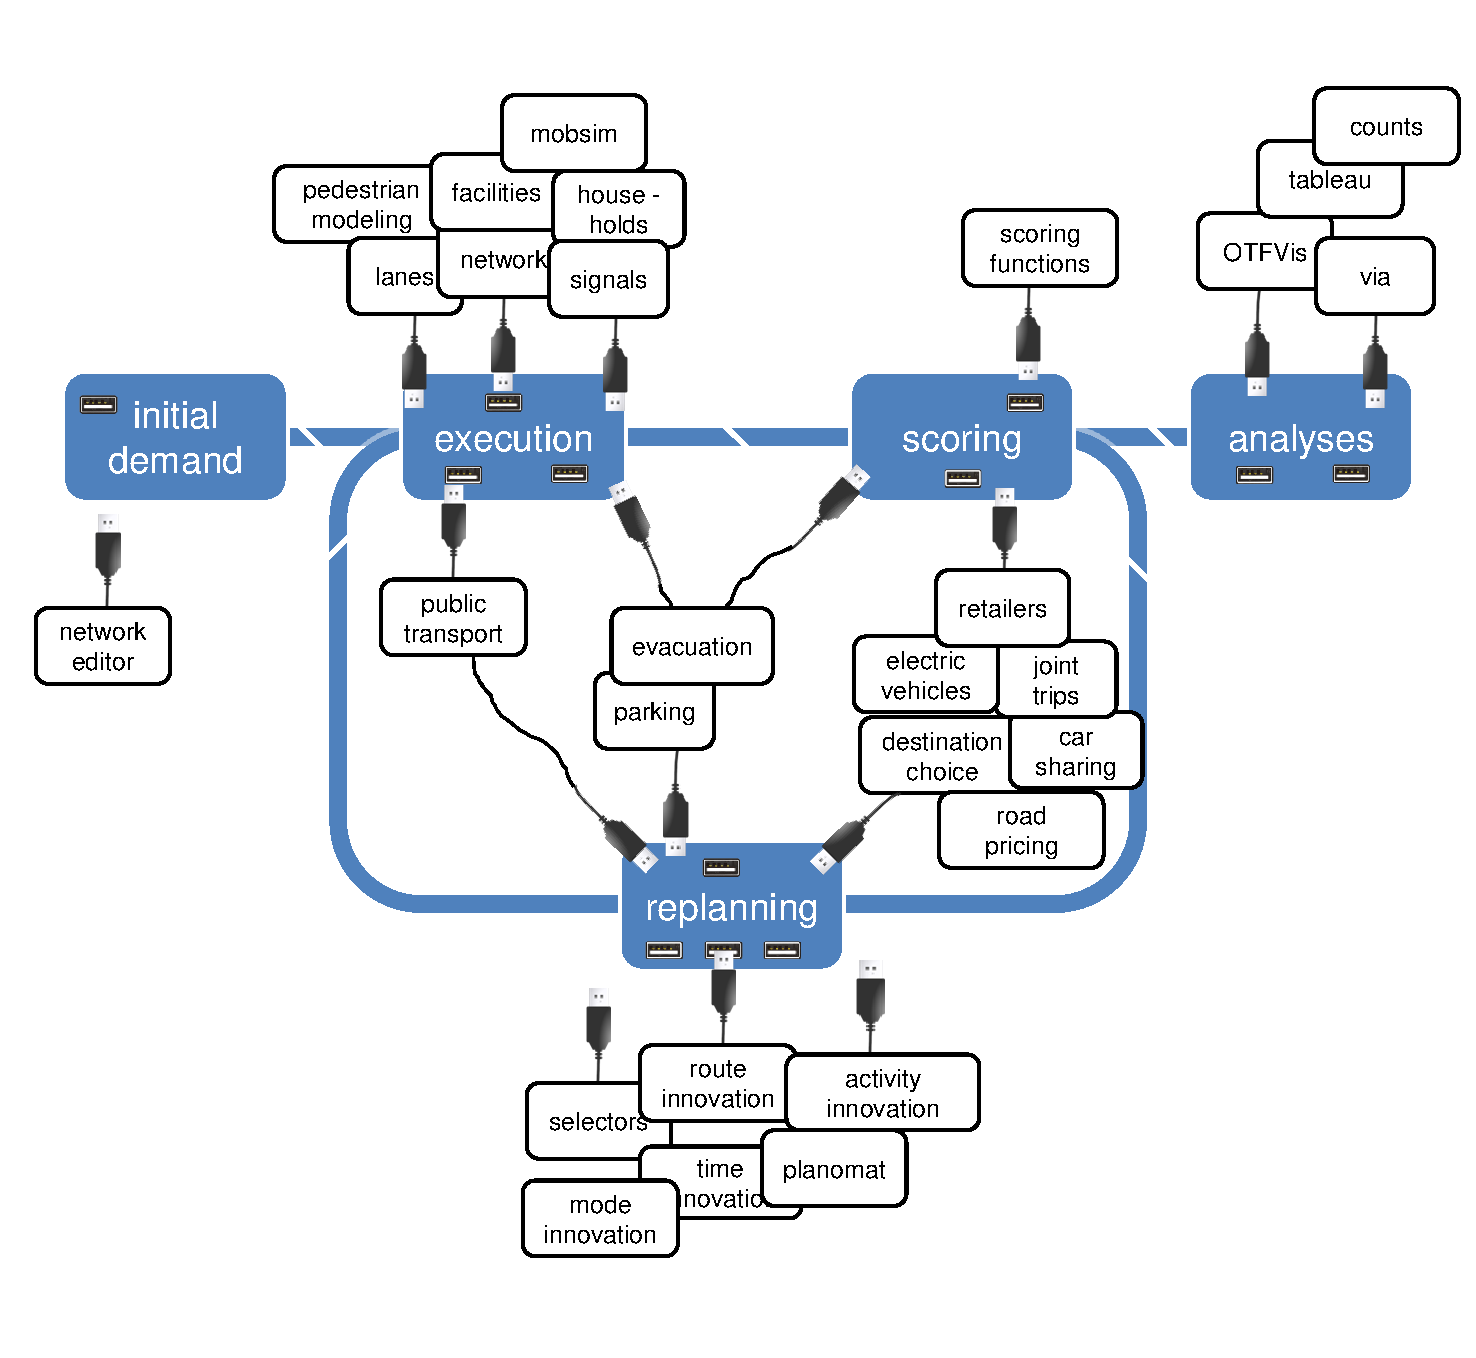
\includegraphics[width=0.99\textwidth, angle=0]{extending/figures/modules.pdf}}%
{}
%
The description of the modules in this and the following chapters is based on the categorization shown in Table~\ref{tab:modules}.
%
%\kai{TODO: macros for section names to re-use for table entries}
%\ah{Mache das später. Denke die jetzige Korrektur hält eine Weile}

\begin{center}
\begin{longtable}{|l|l|}
\label{tab:modules} \\
\caption{MATSim modules}\\
\hline
%\textbf{Module} & \textbf{Described in} \\
%\hline
\endfirsthead
\multicolumn{2}{c}%
{\tablename\ \thetable\ -- \textit{Continued from previous page}} \\
\hline
%\textbf{Module} & \textbf{Described in} \\
%\hline
\endhead
\hline \multicolumn{2}{r}{\textit{Continued on next page}} \\
\endfoot
\hline
\endlastfoot
	\textbf{MATSim Data Containers} & Section~\ref{sec:matsim-containers} \\
	\hline
	Scenario &  Section~\ref{sec:scenario} \\
	Network  & Section~\ref{sec:network} \\
	Counts  & Section~\ref{sec:counts} \\
	Facilities & Section~\ref{sec:facilities} \\
	Population &  Section~\ref{sec:population} \\
	Households &  Section~\ref{sec:households} \\
	Vehicles &  Section~\ref{sec:vehicles} \\
	\hline
	\textbf{Global Modules and Global Aspects} & Section~\ref{sec:globalmodules} \\
	\hline
	Controler &  Section~\ref{sec:controler} \\
	Global &  Section~\ref{sec:global} \\
	Parallel Computing &  Section~\ref{sec:parallelcomputing} \\
	\hline
	\textbf{Mobsims} & Section~\ref{sec:mobsims} \\
	\hline
	QSim &  Section~\ref{sec:qsim} \\
	JDEQSim &  Section~\ref{sec:jdeqsim} \\
	\hline
	\textbf{Scoring} & Section~\ref{sec:scoring} \\
	\hline
	\textbf{Strategy Modules} & Section~\ref{sec:strategymodules} \\
	\hline
	Time Innovation & Section~\ref{sec:timechoice} \\
	Route Innovation & Section~\ref{sec:routechoice} \\
	Mode Innovation & Section~\ref{sec:modechoice} \\
	Selectors & Section~\ref{sec:selectors} \\
	Destination Innovation & Chapter~\ref{ch:destinationchoice} \\
	\hline
	\textbf{Observational Modules} & Section~\ref{sec:observational} \\
	\hline
	Travel Time Calculator & Section~\ref{sec:ttc} \\
	Link Stats & Section~\ref{sec:linkStats} \\
	\hline
	\textbf{Further Modules Possibly Running in a \gls{matsim} Run} & \\
	\hline
	Within-day Replanning & Chapter~\ref{ch:withinday} \\
	Public Transport & Chapter~\ref{ch:pt} \\
	Multi-Modal Simulation & Chapter~\ref{ch:multimodalsim} \\
	Freight Traffic & Chapter~\ref{ch:freight} \\
	Car Sharing & Chapter~\ref{ch:carsharing} \\
	Joint Trips and Social Networks & Chapter~\ref{ch:jointtrips} \\
	Dynamic Transport Systems & Chapter~\ref{ch:dts} \\
	Parking & Chapter~\ref{ch:parking} \\
	Electric Vehicles & Chapter~\ref{ch:elvehicles} \\
	Air Transport & Chapter~\ref{ch:air} \\
	Roadpricing & Chapter~\ref{ch:roadpricing} \\
	Emissions & Chapter~\ref{ch:emissions} \\
	Accessibility & Chapter~\ref{ch:accessibility} \\
	Evacuation & Chapter~\ref{ch:evacuation}  \\
	WagonSim & Chapter~\ref{ch:wagonSim} \\
	Signals and Lanes & Chapter~\ref{ch:signalslanes} \\
	PSim & Chapter~\ref{ch:psim} \\
	\hline
	\textbf{Standalone Tools} & \\ % Out-Of-The-Loop Tools
	\hline
	Senozon via Visualizer & Chapter~\ref{ch:via} \\
	OTFVis Visualizer & Chapter~\ref{ch:otfvis} \\
	Cadyts & Chapter~\ref{ch:cadyts} \\
	\gls{matsim} For UrbanSim & Chapter~\ref{ch:matsim4urbansim} \\	
	Network Editors &  Chapter~\ref{ch:networkeditor} \\
	Interactive Analysis and Decision Support & Chapter~\ref{ch:businessanalytics} \\
\end{longtable}
\end{center}

% ##################################################################################################################
\section{MATSim Data Containers}
\label{sec:matsim-containers}
% ===================================================================================
\subsection{Scenario}
\label{sec:scenario}
\begin{compactitem}
\item Invoking the module: Add the respective config file section.
\item Configuration: \lstinline|scenario| config file section \ah{Hier haben wir doch eine kleine Inkonsistenz zwischen Container und Configuration Section, oder?}
\item Code: \lstinline|org.matsim.core.scenario|
\end{compactitem}

The \lstinline|scenario| module is, on the one hand, a container containing the main components of a scenario such as the \lstinline|config|, the \lstinline|network|, the \lstinline|population|, the \lstinline|facilities|, the \lstinline|transitSchedule|, \lstinline|households| and \lstinline|vehicles|.

The config file section is, on the other hand, used in a slightly different manner. It defines the usage of lanes, signal systems, road pricing, agent knowledges, vehicles, households and public transport. Still a respective config file section is required for every additional functionality. \kai{Ist das genau so?  Ich habe da ehrlich gesagt das genaue Design nie verstanden.  Oft für ein Eintrag in der scenario config group nur dafür, dass die Daten gelesen werden, und sonst passiert gar nichts.  Hm ...  Geradeziehen???}

%% \subsection{Supply-Side Data Containers}
%% \label{sec:supplysidemodules}
% ===================================================================================
\subsection{Network}
\label{sec:network}
\begin{compactitem}
\item Invoking the module: By adding the respective configuration file section, the module is invoked automatically.
\item Configuring: \lstinline|network| config file section
\item Code: \lstinline|org.matsim.core.network|
\end{compactitem}

It is possible to make network attributes time-dependent, as observed in reality in case of accidents or adaptive traffic control, with varying speed limits or driving directions of lanes on multi-lane roads with heavily unbalanced load over the course of a day. Attributes that can be adapted are free speed, number of lanes and flow capacity.

The adaptation can be specified by adding following two lines to the \lstinline|network| configuration file section:
\begin{lstlisting}
<param name="timeVariantNetwork" value="true" />
<param name="inputChangeEventsFile" value="path_to_change_events_file" />
\end{lstlisting}
%
An example file setting the free speed of three network links to zero is as follows:
%
\begin{lstlisting}
<?xml version="1.0" encoding="UTF-8"?>
	<networkChangeEvents xmlns="http://www.matsim.org/files/dtd"
	xmlns:xsi="http://www.w3.org/2001/XMLSchema-instance"
	xsi:schemaLocation="http://www.matsim.org/files/dtd
	http://www.matsim.org/files/dtd/networkChangeEvents.xsd">}

  <networkChangeEvent startTime="03:06:00">
    <link refId="12487"/>
    <link refId="12489"/>
    <link refId="12491"/>
    <freespeed type="absolute" value="0.0"/>
  </networkChangeEvent>

</networkChangeEvents>
\end{lstlisting}
%
Alternatively, network change events can be directly added to the code as follows:
\begin{lstlisting}
networkChangeEvent =
	network.getFactory().createNetworkChangeEvent(...);
networkChangeEvent.setFlowCapacityChange(new ChangeValue(...));
networkChangeEvent.setFreespeedChange(new ChangeValue(...));
networkChangeEvent0.setLanesChange(new ChangeValue(...));
network.addNetworkChangeEvent(networkChangeEvent);
\end{lstlisting}

\kai{lieber ein Verweis auf ein code snippet?  U.a. muss man auf NetworkImpl casten, was wir gerne irgendwann loswerden wollen und daher nicht im Buch haben wollen.}

% ===================================================================================
\subsection{Counts}
\label{sec:counts}
\begin{compactitem}
\item Invoking the module: By adding the respective configuration file section, the module is invoked automatically.
\item Configuration: \lstinline|counts| file section
\item Code: \lstinline|org.matsim.counts|
\end{compactitem}

\gls{matsim} offers the possibility to perform link volume comparisons between simulated and counted value for both motorized individual traffic \citep{Horni_unpub_IVT_2007}  and public transport. The later are described in Chapter \ref{ch:pt}. The count package offers analyses for the average working day with hourly resolution. A google maps based visualization is available, showing each station with a its load curve in a pop-up window at the geographic location.

As shown by \citet[][]{BalmerEtAl_ResRep_bdktzrh_2009}, for the Zürich scenario link volume comparisons have been successfully performed with data based on city level, cantonal level and national level \citep[][]{ASTRA_Webpage_2006}, where an average working day (Monday to Thursday, excluding public holidays) was built. Usually it is helpful to exclude a substantial part of the outer range of the modeled study region to prevent boundary effects.

% ===================================================================================
\subsection{Facilities}
\label{sec:facilities}
\begin{compactitem}
\item Invoking the module: By adding the respective configuration file section, the module is invoked automatically. Please make sure, that added modules can manage facilities.
\item Configuration: \lstinline|facilities| configuration file section
\item Code: \lstinline|org.matsim.core.facilities|
\end{compactitem}

Facilities are a non-mandatory element of \gls{matsim} scenarios. They identify activity locations and can hold opening hour and capacity information. facilities are mostly used in the \gls{matsim} Zürich group, in particular in the Zürich scenario, where facilities are derived from the Federal Enterprise Census 2001 \citep[][]{SwissEnterpriseCensus_manual_2001} providing hectare level information and using NOGA-classification. Detailed technical description of facilities generation is given by \citet[][]{Meister_TechRep_IVT_2008, Meister_unpub_IVT_2007}.

% ===================================================================================

% ##################################################################################################################
%% \subsection{Demand-Side Data Containers}
%% \label{sec:dsm}

% ===================================================================================
\subsection{Population}
\label{sec:population}
\begin{compactitem}
\item Invoking the module: By adding the respective configuration file section, the module is invoked automatically.
\item Configuration: \lstinline|plans| config file section. Optionally the path to a person attributes file in \lstinline|ObjectAttributes| format can be specified.
\item Code: \lstinline|org.matsim.core.population|
\end{compactitem}

The population module manages transport demand, i.e.,\,the population and the agents' plans.
% ===================================================================================
\subsection{Households}
\label{sec:households}
\begin{compactitem}
\item Invoking the module: Enable househlds in the \lstinline|scenario| section of the configuration file and provide the paths to a households file and another file containing the households' attributes in the configuration file section \lstinline|households|.
\item Configuration: \lstinline|households| config file section
\item Code: \lstinline|org.matsim.households|
\end{compactitem}

Similar to the vehicles module, the household module is not used by default in \gls{matsim}.

% ===================================================================================
%% \subsection{Data containers belonging both to demand and to supply}
\subsection{Vehicles}
\label{sec:vehicles}

%% A private household's decision to buy a vehicle in order to satisfy one's transport needs is a demand side decision.
%% %
%% However, if a public transit company decides to buy buses of a certain type, this is more a supply side decision (to supply potential passengers with a vehicle) than a demand side decision (the vehicle will have a demand for road space once it runs).



\begin{compactitem}
\item Invoking the module: Vehicles need to be enabled in the \lstinline|scenario| configuration file section.
\item Configuration: At the moment vehicles are only used for public transport (Chapter~\ref{ch:pt}), i.e.,\,motorized individual traffic vehicles are not used in \gls{matsim} nowadays. Thus, the configuration file section specifying the input file is located in the \lstinline|transit| configuration file section, while the vehicles module does not have its own configuration file section. 
\ah{Klären, ob man diese kleine Inkonsistenz beheben möchte.}  
\kai{Ist das nicht schon erledigt?}
\ah{final String vehiclesFile = this.config.transit().getVehiclesFile();}
\kai{Arghh.}
%
This might change one day when the parking module will start to use vehicles. \citet[][]{JaeggiEtAl_TRR_2012} might serve as an empirical base for the assignment of vehicles to agents or households.
\item Code: \lstinline|org.matsim.vehicles|
\end{compactitem}

The vehicles package provides a file reader and a factory to create vehicles.

%##################################################################################################################
\section{Global Modules and Global Aspects}
\label{sec:globalmodules}
% ===================================================================================
\subsection{Controler}
\label{sec:controler}
\begin{compactitem}
\item Invoking the module: Run \lstinline|org.matsim.run.Controler|
\item Configuration: \lstinline|controler| configuration file section
\item Code: \lstinline|org.matsim.core.controler|
\end{compactitem}

The controler is an indispensable module for running \gls{matsim}. The module, can be furthermore extended by \lstinline|Events| and \lstinline|Listeners| as detailed in Chapter~\ref{ch:extensionpoints}. 
%% Classes implementing one or more \lstinline|Listener Interfaces| and can be registered with the Controler with \lstinline|addControlerListener()|. The controler fires \lstinline|Controler Events| at specific points during the run to the registered \lstinline|Listeners|, which can then execute their own code.
%
%Das ist nur ein Ausschnitt von dem, was der Controler kann.  Da es im entsprechenden Kap. ja beschrieben wird, brauchen wir das hier m.E. nicht nochmal. kai, dec'14

%% \textcolor{gray}{\st{Another possibility to customize the controler is by inheritence from the class} \lstinline|org.matsim.core.controler|.}  \kai{Please do not do or advertise this any more.}

% ===================================================================================
\subsection{Global}
\label{sec:global}
\begin{compactitem}
\item Invoking the module: The module is very sparse and only used to transfer some parameters to the simulation. Add a respective config file section.
\item Configuration: \lstinline|global| config file section. Arguably, this section should be merged with the controler section.
\item Code: \lstinline|org.matsim.core.config.groups.GlobalConfigGroup|
\end{compactitem}

The replanning modules get their information about number of threads from this module. \kai{nicht unter parallel computing?  Wäre meiner Erfahrung nach tatsächlich hilfreich, die paralellen Aspekte zusammenzufassen.}


% ===================================================================================
\subsection{Parallel Computing}
\label{sec:parallelcomputing}
\begin{compactitem}
\item Invoking the module: Define the number of threads in the \lstinline|qsim| and the \lstinline|parallelEventHandling| section
\item Configuration: \lstinline|parallelEventHandling| and \lstinline|qsim| configuration file section
\item Code: mainly \lstinline|org.matsim.core.events.ParallelEventsManagerImpl| for parallel event handling. See qsim for parallel mobsim running.
\end{compactitem}

As described in \citet[][]{WaraichEtAl_TechRep_IVT_2009, WaraichEtAl_STRC_2009} the simulation can be substantially speed-up when using multiple threads for the events handling, usually being a bottleneck in \gls{matsim} simulation runs. Amongst others, in the \lstinline|parallelEventHandling| configuration file section, the number of threads to be used can be specified. 
% Clearly, the number of threads should correspond with available processor cores.  \kai{Meine Erfahrung ist eine andere, und je nach Maschine kann man das manchmal überauslasten und manchmal sollte man es eher unterauslasten.}  
According to our experiences the optimal degree of capacity utilization (threads versus cores) is highly machine-dependent.
As mentioned above, the mobsim \emph{QSim} is running parallel by default.

Being able to speed-up scenarios might become even more important than today, when additional innovation (choice) dimensions are added with large variability in the parameters rendering ensemble runs necessary. % (see Section~\ref{sec:variability}).

%\ah{Marcel hatte mal Testreihe mit Identifikation der Laufzeit einzelner Module (QSim, Eventshandling etc.) geplant. Nachfragen, ob schon was vorhanden}

% ##################################################################################################################
\section{Mobsims}
\label{sec:mobsims}
An overview of \gls{matsim} mobility simulations is given in \citet[][]{Dobler_TechRep_IVT_2011}. See also the presentation of \citet[][]{Rieser_unpub_IVT_2011}.

% ===================================================================================
\subsection{QSim}
\label{sec:qsim}
\begin{compactitem}
\item Invoking the module: Set the parameter \lstinline|mobsim| of \lstinline|controler| config file section to \lstinline|qsim| provide a \lstinline|qsim| config file section.
\item Configuration: \lstinline|qsim| config section
\item Code: \lstinline|org.matsim.core.mobsim.qsim|
\end{compactitem}

At the moment, in most applications \emph{QSim} \citep[][]{Dobler_TechRep_IVT_2011, Dobler_STRC_2010} is used. 
%% It has started as a software branch of \emph{queueSimulation} before supplanting this later simulation. 
Through multiple engines it can be run in parallel and simulate multi-modal traffic (Chapter~\ref{ch:multimodalsim}). It is queue-based and time-step based. The simulation is able to handle time-variant networks, within-day replanning \citep[][]{Dobler_TechRep_IVT_2009}, public transport \citep[][]{Rieser_PhDThesis_2010} and in an experimental manner also traffic lights \citep[][]{Neumann_MastersThesis_2008}). Inclusion of public transport is described in Chapter~\ref{ch:pt}.

% ===================================================================================
\subsection{JDEQSim}
\label{sec:jdeqsim}
\begin{compactitem}
\item Invoking the module: Set the parameter \lstinline|mobsim| of \lstinline|controler| config file section to \lstinline|JDEQSim| provide a \lstinline|jdeqsim| config file section.
\item Configuration: \lstinline|jdeqsim| config file section
\item Code: \lstinline|org.matsim.core.mobsim.jdeqsim|
\end{compactitem}

\gls{jdeqsim} \citep[][]{WaraichEtAl_TechRep_IVT_2009, WaraichEtAl_STRC_2009} was used for project \emph{KTI Frequencies} \citep[][]{BalmerEtAl_ResRep_datapuls_2010}. It is is a \gls{java} reimplementation of \gls{deqsim} \citep[][]{WaraichEtAl_STRC_2009, CharyparEtAl_TRR_2007, CharyparEtAl_TRB_2009} and provides parallel event handling but no parallel simulation \citep[][p.11]{BalmerEtAl_ResRep_datapuls_2010}. Back-propagating gaps are supported. Traffic lights, public transport and within-day replanning are not supported.

%##################################################################################################################
\section{Scoring}
\label{sec:scoring}
\begin{compactitem}
\item Invoking the module: add below section to config file
\item Configuration: \lstinline|planCalcScore| config file section
\item Code: \lstinline|org.matsim.core.scoring|
\end{compactitem}
%
The parameters related to scoring described in Chapter~\ref{ch:scoring}.

% ===================================================================================

%##################################################################################################################
\section{Strategy Modules}
\label{sec:strategymodules}
%\kai{Habe ``strategy'' ans Ende gezogen, weil ein matsim run so auch tatsächlich losgeht: erst mobsim, dann scoring, dann replanning.  Gibt es Argumente für andere Reihenfolgen?} \ah{nein, super Punkt!}
The strategy modules are the basic innovation modules available in \gls{matsim}. We do not call them \emph{choice} modules although they are involved in people's choice making. The choice process, however, is performed over the iterations with an \emph{implicit} choice set and it is not based on explicit probability function drawing. Usually, innovation modules also do no define their own utility function. This is particularly true for random mutation modules, where best response modules such as destination innovation are closer to the standard procedure of choice modeling but still not full-blown choice models. For a detailed discussion of \gls{matsim} in choice modeling context see Chapter~\ref{ch:discretechoice}.

All strategy modules are called by configuring the strategy module in the configuration file as shown in the following example.
%
\begin{lstlisting}
<module name="strategy" >
    <param name="ModuleProbability_1" value="0.1" />
    <param name="Module_1" value="ChangeLegMode" />
    <param name="ModuleProbability_2" value="0.2" />
    <param name="Module_2" value="TimeAllocationMutator" />
    <param name="ModuleProbability_3" value="0.7" />
    <param name="Module_3" value="SelectExpBeta" />
</module>
\end{lstlisting}
%
\kai{Hier gibt es eine neue, bessere Syntax.  NB dass wir da gerade noch am ``Verhandeln'' sind!}
%
Strategy modules are numbered, where each module is given a weight which determines the probability by which the course of action represented by the module is taken. In this example, each agent changes his leg mode with probability 0.1, its plan timing with probability 0.2. A strategy module is, in the code, always a combination of a plan selector and zero or more strategy module elements. In the example, the agent chooses a plan from his set of plans according to a logit model with probability 0.7. The weights of the strategy modules are renormalized in case they do not sum to one.

By specifying the parameter \lstinline|ModuleSubpopulation_X|, i.e.,\,\lstinline|<param name="ModuleSubpopulation_1" value="externalAgent"/>| replanning strategies can be applied to distinct sub-populations.

%Combining different modules is not straight-forward in MATSim. This important topic urgently awaits future analysis. To begin with, here, the combination of the strategy modules with public transport is presented in Table \ref{tab:combination}.
%
%% ----------------------------------
%\createtable%
%{Strategy Module Combination}%
%{Strategy Module Combination}%
%{\label{tab:combination}}%
%{%
  %\begin{tabular}[c]{|c|c|c|}
   %\hline
%\textbf{Innovation Dimension}	& \textbf{Default Strategy} & \textbf{Public Transport}\\
%\hline
%time innovation & TimeAllocationMutator &  TransitTimeAllocationMutator\\
%\hline
%route innovation & ReRoute & ReRoute \\
%\hline
%mode innovation & \multirow{2}{*}{ChangeLegMode} & \multirow{2}{*}{TransitChangeLegMode} \\
%(all legs get same mode) &  &  \\
%\hline
%mode innovation & \multirow{2}{*}{ChangeSingleLegMode} & \multirow{2}{*}{TransitChangeSingleLegMode} \\
%(each leg can have a different mode) &  &  \\
%\hline
%mode innovation & \multirow{2}{*}{SubtourModeChoice} & \multirow{2}{*}{TransitSubtourModeChoice} \\
%(subtour-based) &  &  \\
%\hline
%destination innovation & LocationChoice & LocationChoice \\
%\hline
  %\end{tabular}
%}%
%{}

\kai{Ich meine, dass es diese Transit Sonderformen gar nicht mehr gibt.  ????} 

\ah{Please note, that combining strategy modules that are \gls{contribution} such as destination innovation or public transport is not straight forward. Contact the mailing list, for further information.}

% ===================================================================================
\subsection{Time Innovation}
\label{sec:timechoice}
\begin{compactitem}
\item Invoking the module: Time choice is applied by defining its parameters in the configuration file and by adapting the configuration file strategy module as follows
%
\begin{lstlisting}
<module name="strategy" >
    <param name="ModuleProbability_1" value="0.x" />
    <param name="Module_1" value="TimeAllocationMutator" />
    [...]
</module>
\end{lstlisting}
%
\item Configuration: \lstinline|TimeAllocationMutator| config file section
\item Code: \lstinline|org.matsim.core.replanning.modules.TimeAllocationMutator|
\end{compactitem}

The module shifts activity end times randomly within a configurable range as described by \citet[][]{BalmerEtAl_Timmermans_2005, Raney_PhDThesis_2005, Balmer_unpub_VSP_2004, BalmerEtAl_unpub_EIRASS_2004, BalmerEtAl_unpub_STRC_2004}. A best-reponse approach to time choice is applied by "Planomat" described in Section~\ref{sec:planomat}.

% ===================================================================================
\subsection{Route Innovation}
\label{sec:routechoice}
\begin{compactitem}
\item Invoking the module: Route choice is applied by defining its parameters in the configuration file and by adapting the configuration file strategy module as follows
%
\begin{lstlisting}
<module name="strategy" >
    <param name="ModuleProbability_1" value="0.x" />
    <param name="Module_1" value="ReRoute" />
    [...]
</module>
\end{lstlisting}
%
\item Configuration: \lstinline|planscalcroute| config file section. The routing algorithm needs to be specified in the configuration file controler module
%
\begin{lstlisting}
<module name="controler" >
    <param name="routingAlgorithmType" value="{Dijkstra | FastDijkstra |
    		AStarLandmarks | FastAStarLandmarks}" />
    [...]
</module>
\end{lstlisting}
\item Code: \lstinline|org.matsim.core.router|
\end{compactitem}
%
\gls{matsim} routing is described by \citet[]{LefebvreBalmer_STRC_2007, LefebvreBalmer_TechRep_IVT_2007}. The configuration necessary for public transport is shown in Chapter \ref{ch:pt}.  \kai{Da steht m.E.\ noch nichts in der Richtung.  Aber meiner Erinnerung nach ist auch gar keine Sonderkonfiguration mehr nötig.  Michael Z.?}

% ===================================================================================
\subsection{Mode Innovation}
\label{sec:modechoice}
\begin{compactitem}
\item Invoking the module: Mode choice is applied by defining its parameters in the configuration file and by adapting the configuration file strategy module by choosing one of the mode choice options as follows
\begin{lstlisting}
<module name="strategy" >
    <param name="ModuleProbability_1" value="0.x" />
    <param name="Module_1" value="{ChangeLegMode |
    		ChangeSingleLegMode | SubtourModeChoice}" />
    [...]
</module>
\end{lstlisting}
%
\item Configuration: Corresponding with the chose type of mode choice a respective config file section needs to be added:
%
\begin{lstlisting}
<module name="{changeLegMode |
				changeLegMode | subtourModeChoice}" >
    <param name="param0" value="value0" />
    [...]
</module>
\end{lstlisting}
%
\item Code: \lstinline|org.matsim.core.replanning.modules| and \lstinline|org.matsim.population.algorithms|.
\end{compactitem}

\lstinline|ChangeLegMode| randomly picks one of the plans of a person and changes its mode of transport. By default, the supported modes are driving a car and using public transport. Only one mode of transport per plan is supported. For using different modes for sub-tours on a single day the \lstinline|SubtourModeChoice| module is required. Optionally, car-availability is respected. \lstinline|ChangeSingleLegMode| randomly picks one of the plans of a person and changes the mode of transport of one single leg. The leg is picked randomly. In contrast to \lstinline|ChangeLegMode|, it allows for multiple modes in one plan. By default, the supported modes are driving a car and using public transport. Also, this module is able to (optionally) respect car-availability.

Mode choice is described by \citet[][]{RieserEtAl_TRR_2009, MeisterEtAl_WCTRS_2010, CiariEtAl_STRC_2008, CiariEtAl_STRC_2007}.

% ===================================================================================
\subsection{Selectors}
\label{sec:selectors}
\begin{compactitem}
\item Invoking the module: Define one of the available selectors in the configuration file strategy module as follows
%
\begin{lstlisting}
<module name="strategy" >
    <param name="ModuleProbability_1" value="0.x" />
    <param name="Module_1" value="{a specific selector}" />
    [...]
</module>
\end{lstlisting}
%
Following selectors are available in the configuration file strategy module:
%
\begin{compactitem}
	\item \lstinline|KeepLastSelected| keeps the plan selected in the previous iteration.
	\item \lstinline|BestScore| selects the plan with the highest score of the previous iteration.
	\item \lstinline|SelectExpBeta| performs \gls{mnl} selection between plans.
	\item \lstinline|ChangeExpBeta| changes to a different plan with probability dependent on $e^{\Delta_{score}}$, where $\Delta_{score}$ is the score difference between the two plans.
	\item \lstinline|SelectRandom| performs random selection between the plans.
	\item \lstinline|SelectPathSizeLogit| selects an existing plan according to the path size logit described by \citet[][]{FrejingerBierlaire_TransResB_2007}.
\end{compactitem}
%
\item Configuration: no further configuration necessary \ah{? selectExpBeta ...}
\item Code: \lstinline|org.matsim.core.replanning.selectors|
\end{compactitem}

Note, that the \lstinline|BestScore| should be used with care as it is prone to getting stuck with sub-optimal plans. Plans that are rated bad due to a random fluctuation in one single iteration, due to e.g.,\,a rare traffic jam, will never be tested again. It is therefore recommended to use this in conjunction with \lstinline|SelectRandom| only.

Besides the selectors for plan modification and execution, in the near future also the plan remover will be available for configuration. Per default, the plan with the lowest score is removed if the agent's memory is full. In line with the requirements of e.g.,\,simulated annealing approaches, the removal of candidates will be configurable to be probabilistically dependent on the plan score similar to the selection in \lstinline|SelectExpBeta|. This will reduce the probability to get stuck with sub-optimal plans, that were dominant in earlier iterations.
\ah{siehe Mail by M. Zilske, August 14 ``[Matsim-devel] custom plan selector for removal'')}

%##################################################################################################################
\section{Observational Modules}
\label{sec:observational}

% ===================================================================================
\subsection{Travel Time Calculator}
\label{sec:ttc}
\begin{compactitem}
\item Invoking the module: The module is invoked by specifying the respective configuration file section.
\item Configuration: \lstinline|travelTimeCalculator| config file section
\item Code: \lstinline|org.matsim.core.trafficmonitoring|
\end{compactitem}

The routing module, as an example, needs travel time estimations for all links of the network. To keep the computational effort feasible, the travel time estimations need to aggregated to time bins. The parameters of this aggregation, such as the bin size, can be specified in the configuration file section \lstinline|travelTimeCalculator|.

% ===================================================================================
\subsection{Link Stats}
\label{sec:linkStats}
\begin{compactitem}
\item Invoking the module: The module is invoked by specifying the respective configuration file section.
\item Configuration: \lstinline|linkStats| configuration file section
\item Code: \lstinline|org.matsim.analysis.CalcLinkStats|
\end{compactitem}

Link stats allow to specify the output interval of simulation statistics of individual links. They are amongst other, used for the comparison with count values. It is configurable, if the simulated volumes should be written per iteration or averaged over multiple iterations.

% ##################################################################################################################
\section{MATSim Survival Guide}
\label{sec:survival}
There are already many options and possibilities available with \gls{matsim}, and finding them can be a taunting exercise.  Here are a couple of recommendations, derived from our own frequent use of the system.
\begin{enumerate}

\item Always start and test with a small example.

\item Always test large scenarios with one percent runs first (e.g.,\,a randomly drawn 1\,\% subsample of your initial demand).

\item Check \lstinline{logfileWarningsErrors.log}.

\item Check the comments that are attached to the config options.

One finds them in the file \lstinline{output_config.xml.gz}, or near the beginning of \lstinline{logfile.log}.

\item Search for documentation via \url{http://matsim.org/javadoc}.

\end{enumerate}


% ##################################################################################################################
% Local Variables:
% mode: latex
% mode: reftex
% mode: visual-line
% TeX-master: "../../main"
% comment-padding: 1
% fill-column: 9999
% End: 
